\documentclass[]{article}
\usepackage[top=2cm,left=1cm, right=1cm, bottom=2cm]{geometry}
\usepackage{amsmath}
\usepackage{graphicx}
\usepackage{natbib}
\usepackage{apalike}
\usepackage{mathtools}
\bibliographystyle{abbrvnat}
\setcitestyle{authoryear, open={(},close={)}}

%opening
\title{Equations for a growing (and thickening) cambial cell with a multilayered wall including the effect of cellulose microfibrils reorientation}
\author{Cyril Bozonnet, Tancrède Alméras, Joseph Gril, Félix Hartmann}

\begin{document}
	
	\maketitle
	\section{Main objective}
Explore the effect  of the wall heterogeneity on the growth of a cambial cell.
	
	\section{Geometry and kinematics}
	\subsection{At the cell scale}
	\begin{figure}[h]
		\centering
		{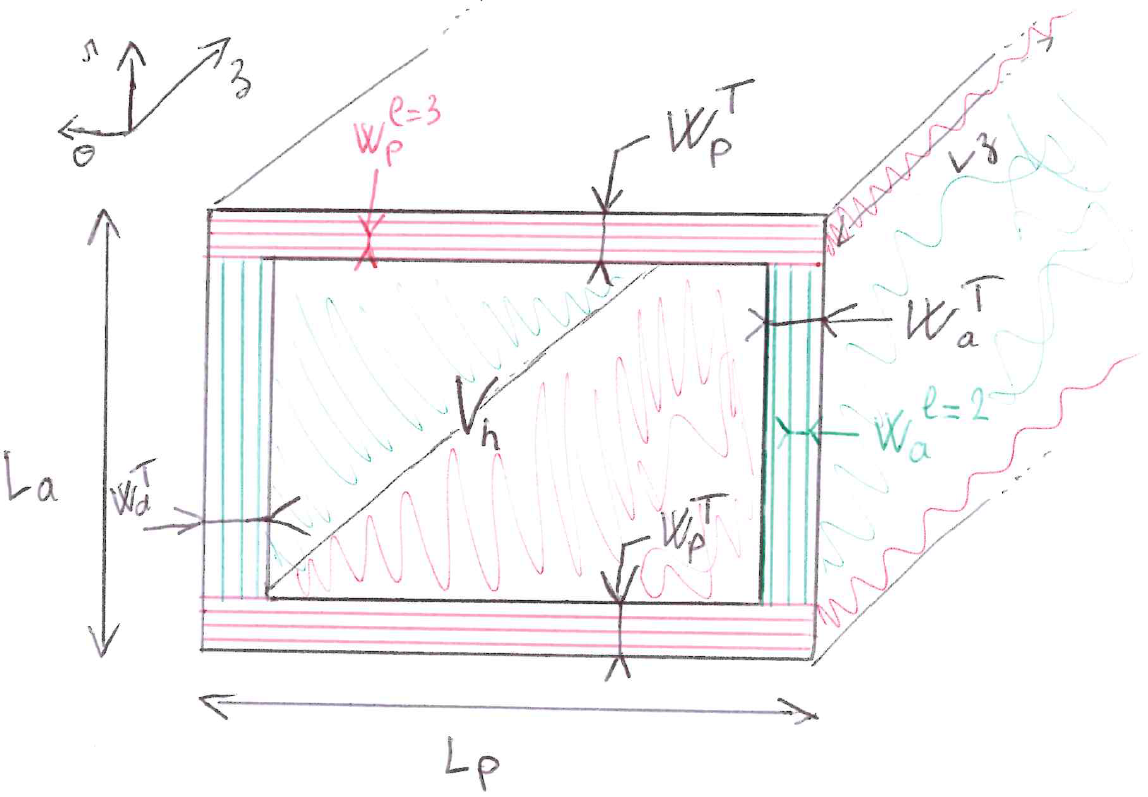
\includegraphics[width=0.5\textwidth]{schema.png}}
		\caption{Geometry and notations. The reference frame at the top left corner shows the link between the present geometry and the one of an actual cambial cell whose growth would be mainly along $r$.}
		\label{fig1}
	\end{figure}
	The geometry of the cambial cell is displayed in figure \ref{fig1}. 
	We make the following additional assumptions:
	\begin{itemize}
		\item Growth occurs only along $r$
		\item Wall layer deposition occurs only along the anticlinal walls
		\item Wall synthesis is regulated so that the total anticlinal wall thickness is constant
	\end{itemize}
Under the previous hypothesis, the elongation rate in the radial (anticlinal) direction is
\begin{equation}\label{ER}
	\boxed{
	\dot{\varepsilon}_a = \frac{1}{V_h}\frac{{\rm d} V_h}{{\rm d} t} =  \frac{Q}{V_h} = \frac{A \kappa_h}{V_h}\left(\Psi_{src} -P + \Pi \right)},
\end{equation}
where $V_h$ is the lumen volume, $Q$ the sum of water fluxes entering or leaving the cell, $A$ the exchange area for the water fluxes, $\kappa_h$ the hydraulic conductivity, $\Psi_{src}$, $P$, and $\Pi$ are the total external, the cell pressure and cell osmotic potentials, respectively. The cell pressure is computed from the mean anticlinal stresses, $\overline{\sigma_a}$, as
\begin{equation}
	P=\frac{2\overline{\sigma_a}W_a^T}{L_p}.
\end{equation}

\subsection{At the wall scale}
The wall structure is formed by multiple layers spreaded onto each other. Each layer is made up of cellulose microfibrils (MF), that are inclined at an angle $\phi$ with respect to the longitudinal direction, and surrounded by a gel composed of different polymers. These MF are deposited at a given angle, $\phi_0^i$. The MF angle in a wall layer $\phi^i$ evolves with the total wall layer deformation, $\varepsilon_T^i$ according to
\begin{equation}
	\boxed{
	{\rm tan}(\phi^i) = {\rm tan}(\phi_0^i)\exp{(\varepsilon_T^i)}}.
\end{equation}
The total layer deformation is computed as $\varepsilon_T^i=(L_a-L_0^i)/L_0^i$, where $L_0^i$ is the length of the layer when it was deposited and $L_a$ is the actual anticlinal cell length (obtained by integrating Eq. (\ref{ER})).

\section{Mechanics of a growing heterogeneous cell wall}
\subsection{General procedure}
In order to describre properly the behaviour of this heterogeneous medium we proceed in different steps:
\begin{enumerate}
	\item From the cell boundary conditions and the kinematics, we know the deformation rate tensor in the reference frame ($R$,$Z$) for each layer.
	\item Through a first rotation step (of angle $\pi/2-\phi^i$), one can express the previous tensor in the MF frame of each layer ($1$,$2$)$^i$.
	\item Appplying a consitutive equation, one can then obtain the changes in the stress fields in each layer in the MF frame $(\dot{\sigma_1}$,$\dot{\sigma_2}$,$\dot{\tau_{12}})^i$. The consitutive equation will take into account the heterogenous nature of the wall layer.
	\item Through  a second rotation step (of angle $\phi^i-\pi/2$), one can express the changes in the stress fields from the rotated frame to the reference frame, for each wall layer, and integrate them to get the stress fields.
	\item Finally, the mean anticlinal wall stress can be computed, frow which one can compute the new pressure, that will then be used to compute the new elongation rate.
\end{enumerate}
This procedure is not restricted to mono-dimensional growth and could be applied in case of intrusive growth as well.
\subsection{Deformation rate tensor}
Assuming that the cell deformation is blocked in the longitudinal direction, that there is no distortion in the ($R$,$Z$) frame, the cell deformation rate tensor can be written, in a vector form,
\begin{equation}
	\boxed{
	\bar{\bar{\varepsilon}}_{R,Z}= \left(\begin{matrix}
		\dot{\varepsilon}_R\\
		\dot{\varepsilon}_Z\\
		\dot{\gamma}_{RZ2}
	\end{matrix}\right)
=
\left(\begin{matrix}
	\dot{\varepsilon}_a\\
	0\\
	0
\end{matrix}\right)}.
\end{equation}
This expression is true for all wall layers.
\subsection{Rotation steps}
The elongation rate tensor in a wall layer can be expressed in the rotated frame (rotation of angle $\theta$) through the following operation  
\begin{equation}
	\left(\begin{matrix}
		\dot{\varepsilon}_1\\
		\dot{\varepsilon}_2\\
		\dot{\gamma}_{12}
	\end{matrix}\right)^i
=
R_{\varepsilon}(\theta^i)
\left(\begin{matrix}
	\dot{\varepsilon}_a\\
	0\\
	0
\end{matrix}\right),
\end{equation}
with (\citet{aga17}, p190)
\begin{equation}
R_{\varepsilon}(\theta)
	=
	\left(\begin{matrix}
	\cos^2(\theta) & \sin^2(\theta) & \sin(\theta)\cos(\theta)\\
	\sin^2(\theta) & \cos^2(\theta) & -\sin(\theta)\cos(\theta)\\
	-2\sin(\theta)\cos(\theta) & 2\sin(\theta)\cos(\theta) & \cos^2(\theta)-\sin^2(\theta)
\end{matrix}\right)
,
\end{equation}
and $\theta^i=\pi/2-\phi^i$.

The stress tensor components in the reference frame can be computed from the stress tensor components in the MF frame using 
\begin{equation}
	\boxed{
	\left(\begin{matrix}
		\dot{\sigma}_a\\
		\dot{\sigma}_Z\\
		\dot{\tau}_{RZ}
	\end{matrix}\right)^i
	=
R_{\sigma}(\theta^i)
	\left(\begin{matrix}
	\dot{\sigma}_1\\
	\dot{\sigma}_2\\
	\dot{\tau}_{12}
\end{matrix}\right)^i},
\end{equation}
with (\citet{aga17}, p190) 
\begin{equation}
	R_{\sigma}(\theta)
	=
	\left(\begin{matrix}
		\cos^2(\theta) & \sin^2(\theta) & 2\sin(\theta)\cos(\theta)\\
		\sin^2(\theta) & \cos^2(\theta) & -2\sin(\theta)\cos(\theta)\\
		-\sin(\theta)\cos(\theta) & \sin(\theta)\cos(\theta) & \cos^2(\theta)-\sin^2(\theta)
	\end{matrix}\right)
	,
\end{equation}
and $\theta^i=\phi^i-\pi/2$.
\subsection{Constitutive equation}
\subsubsection{General form}
We assume that the mechanical behaviour of the ensemble fibre + gel within each wall layer is similar to a Bingham fluid and that we are in plane stress conditions, i.e.,
\begin{equation}\label{constitutive}
	\boxed{
		\left(\begin{matrix}
		\dot{\sigma}_1\\
		\dot{\sigma}_2\\
		\dot{\tau}_{12}
	\end{matrix}\right)^i
=
\overline{\overline{Q}}
	\left(\begin{matrix}
	\dot{\varepsilon}_1\\
	\dot{\varepsilon}_2\\
	\dot{\gamma}_{12}
\end{matrix}\right)^i
- \frac{1}{\tau_{visc}}	
\left[
\left(\begin{matrix}
	{\sigma}_1\\
	{\sigma}_2\\
	{\tau}_{12}
\end{matrix}\right)^i
-
\left(\begin{matrix}
	\beta_1\\
	\beta_2\\
	\beta_{12}
\end{matrix}\right)^i
\right]^+},
\end{equation}
where $\overline{\overline{Q}}$ is the rigidity tensor in plane stress conditions (it is the same for all layers), $\tau_{visc}$ is the characteristic viscous time (supposedly the same for all stress components), $\beta_1$, $\beta_2$ and $\beta_{12}$ are the different yield thresholds, and the $(x)^+$ notation is equivalent to ${\rm max} (x,0)$.
The rigidity tensor under plane stress hypothesis is expressed as
\begin{equation}
	\overline{\overline{Q}}=
	\left(\begin{matrix}
		Q_{11} & Q_{12} & 0\\
		Q_{12} & Q_{22} & 0\\
		0 & 0 & Q_{66}
	\end{matrix}\right)=
	\left(\begin{matrix}
	\frac{E_1}{1-\nu_{12}\nu_{21}} & \frac{\nu_{21}E_1}{1-\nu_{12}\nu_{21}} & 0\\
	\frac{\nu_{21}E_1}{1-\nu_{12}\nu_{21}} & \frac{E_2}{1-\nu_{12}\nu_{21}} & 0\\
	0 & 0 & G_{12}
\end{matrix}\right),
\end{equation}
where $E_1$, $E_2$, $\nu_{12}$, $\nu_{21}$ and $G_{12}$, are the Young's modulus, Poisson coefficients, and the shear modulus in the MF frame, respectively.

\subsubsection{Elastic parameters}
To compute the elastic coefficients of the fibre + gel (matrix) ensemble, we use the Halpin-Tsai equations, that are widely used to predict the elastic properties of polymers reinforced by short fibers \citep{halpin76,abrate86}. One can thus compute the elastic properties using the following expressions:
\begin{align}
	E_1 &= E_m \frac{1+\xi \frac{l}{d} \eta_L V_f}{1-\eta_LV_f}, \nonumber \\
	E_2 &= E_m \frac{1+\xi \eta_T V_f}{1-\eta_TV_f},  \nonumber \\
	G_{12} &= G_m \frac{1+\xi \eta_G V_f}{1-\eta_GV_f}, \nonumber\\
	\nu_{12}&=  \nu_m \frac{1+\xi \eta_\nu V_f}{1-\eta_\nu V_f}, \nonumber\\
	\nu_{21}& = \nu_{12}\frac{E_2}{E_1},  \\
	{\rm where \  } \eta_L & = \frac{(E_f/E_m - 1)}{E_f/E_m + \xi l/d}, \nonumber\\
	\eta_T & = \frac{(E_f/E_m - 1)}{E_f/E_m + \xi }, \nonumber \\
	\eta_G & = \frac{(G_f/G_m - 1)}{G_f/G_m + \xi }, \nonumber \\
	{\rm and \  } \eta_\nu & = \frac{(\nu_f/\nu_m - 1)}{\nu_f/\nu_m + \xi }. \nonumber
\end{align}
The different parameters, their significance and indicative values are reported in table 1.
\begin{center}	
	\begin{table}\label{table1}
		\centering
		\begin{tabular}{llll}                                                                    
			Variable name      & Description                      & Unit  & Value or expression  \\
			\hline\hline 
			\multicolumn{4}{c}{Material and geometrical properties}\\
			$E_m$                 & Matrix Young's modulus                      & GPa  & 0.01    \\  
			$E_f$                 & MF Young's modulus                    & GPa & 198 \citep{son21}    \\  
			$\nu_m$                  & Matrix Poisson coefficient                       & -  & 0.25    \\
			$\nu_f$            & MF Poisson coefficent & - & 0.22  \citep{son21}      \\
			$G_m$ & Matrix shear modulus & GPa & $E_m/(2(1+\nu_m))$ \\
			$G_f$ & MF shear modulus & GPa & 6.06 \citep{son21} \\
			$V_{f}$        & MF volume fraction     & - & 0.1      \\
			$\xi$        & Reinforcement parameter     & - & 1.5 (for random organization)      \\
			$l/d$        & MF aspect ratio     & - & $10^2$     \\
			\hline
			\multicolumn{4}{c}{Elastic parameters computed from Halpin-Tsai equations using above values}\\
			$E_1$                 & Axial Young's modulus                     & MPa  & 176.3    \\  
			$E_2$                 & Transverse Young's modulus                    & MPa & 12.77  \\  
			$\nu_{12}$                  & Poisson coefficient                       & -  & 0.2911   \\
			$\nu_{21}$            & Poisson coefficient   & - & 0.02 \\
			$G_{12}$            & Shear modulus   & MPa & 4.9 \\
		\end{tabular}
		\caption{Elastic parameters}
	\end{table}
\end{center}
\subsubsection{Plastic thresholds}
Finally, one must compute $\beta_1^i$, $\beta_2^i$ and $\beta_{12}^i$, the plastic thresholds that appear in Eq. (\ref{constitutive}).
To determine whether or not the stresses are above the yield threshold, one must use in the MF frame a criterion adapted to the anisotropic nature of the wall material. For this, we use the Tsai-Hill criterion, that has been widely used for anisotropic composite materials \citep{tsai65, fuc06, mor15}. This criterion states that when the following inequality is violated, plasticity starts:
\begin{equation}\label{tsai_hill}
	\left(\frac{\sigma_1^i}{Y_1}\right)^2 - \frac{\sigma_1^i \sigma_2^i}{Y_1^2} + \left(\frac{\sigma_2^i}{Y_2}\right)^2 + \left(\frac{\tau_{12}^i}{Y_{12}}\right)^2 <1.
\end{equation}
In the previous equation, $Y_1$ and $Y_2$ are the tensile or compressive yield stress in the 1 and 2 directions, and $Y_{12}$ is the shear yield stress. In the $(\sigma_1$, $\sigma_2$, $\tau_{12})^i$ space, this inequality defines an ellipsoid or a sphere, depending on the $Y_1$, $Y_2$ and $Y_{12}$ values, whose surface is the border between elastic and plastic regimes. 

Assuming that the different yield stresses can be computed from the elastic theory using an isotropic strain threshold, one obtains
\begin{equation}
	\left(\frac{\sigma_1^i}{Q_{11}}\right)^2 - \frac{\sigma_1^i \sigma_2^i}{Q_{11}^2} + \left(\frac{\sigma_2^i}{Q_{22}}\right)^2 + \left(\frac{\tau_{12}^i}{Q_{66}}\right)^2 <\varepsilon_0^2,
\end{equation}
where $\varepsilon_0$ is the strain threshold. 

Computing the $\beta_1^i$, $\beta_2^i$ and $\beta_{12}^i$ values is then done as follows:
\begin{itemize}
	\item Knowing the different stress components as well as the different parameters ($\varepsilon_0$,$Q_{11}$,...), one can check whether or not the previous inequality has been violated, i.e., whether the current location in the $(\sigma_1$, $\sigma_2$, $\tau_{12})^i$ space is outside the ellipsoid or not.
	\item If it is outside, the three yield parameters, $\beta_1^i$, $\beta_2^i$ and $\beta_{12}^i$, can be found by taking the orthogonal  projection of the current location in the $(\sigma_1$, $\sigma_2$, $\tau_{12})^i$ space onto the ellispoid, which is equivalent to finding the shortest distance between the point and the ellispoid. This procedure is described in the next section.
	\item Once the yield parameters are known, one can use them in Eq. (\ref{constitutive}) in order to compute the stress changes.
\end{itemize} 
\subsection{Projection onto an ellipsoid}

Here we find the location of a point in the ($\sigma_1$, $\sigma_2$, $\tau_{12}$)$^i$ space that would lie onto the ellispoid defined by Eq. (\ref{tsai_hill}), and minimize the distance with the known stress values.  We first explain the solution for an ``ideal'' ellispoid (in which there is no $\sigma_1\sigma_2$ product), and then explain the change of variable that is necessary to use this solution in our case.

\subsubsection{The case of an ideal ellispoid}
Let $x=(x_1,x_2,x_3)$ being a point onto the surface of an ellispoid whose equation is
\begin{equation}\label{ellipsoid}
	g(x)=\left(\frac{x_1}{a_1}\right)^2+\left(\frac{x_2}{a_2}\right)^2+\left(\frac{x_3}{a_3}\right)^2-1 =0.
\end{equation}
 Let $y=(y_1,y_2,y_3)$ being a point located outside the ellipsoid. The squared distance function between $x$ and $y$ is
 \begin{equation}
 	d(x) =(x_1-y_1)^2 + (x_2-y_2)^2 + (x_3-y_3)^2.
 \end{equation} 
Our goal is to find $x$ that minimizes $d(x)$ while satisfying $g(x)=0$.

 At the minimal or maximal distance, the normal vectors to $d(x)$ and $g(x)$ are parallel, i.e., 
\begin{equation}
	\nabla d(x) = \lambda \nabla g(x),
\end{equation}
where $\lambda$ is a Lagrange multiplier (a scalar). The previous equation can be expressed for all variables,
\begin{align}
	\frac{{\rm d} d(x)}{{\rm d} x_1} & =\lambda\frac{{\rm d} g(x)}{{\rm d} x_1}, \nonumber \\
	\frac{{\rm d} d(x)}{{\rm d} x_2} & =\lambda\frac{{\rm d} g(x)}{{\rm d} x_2}, \\
	\frac{{\rm d} d(x)}{{\rm d} x_3} & =\lambda\frac{{\rm d} g(x)}{{\rm d} x_3}, \nonumber 
\end{align}
which gives the expression of $x$ as a function of $y$, $\lambda$ and the ellipsoid parameters,
\begin{align}
	x_1 & =\frac{y_1}{1-\lambda/a_1^2}, \nonumber \\
	x_2 & =\frac{y_2}{1-\lambda/a_2^2}, \\
	x_3 & =\frac{y_3}{1-\lambda/a_3^2}. \nonumber 
\end{align}
These solutions can then be plugged into the constraint $g(x)=0$, which gives
\begin{equation}
	g(\lambda)=\frac{y_1^2}{a_1^2(1-\lambda/a_1^2)^2}+\frac{y_2^2}{a_2^2(1-\lambda/a_2^2)^2}+\frac{y_3^2}{a_3^2(1-\lambda/a_3^2)^2} -1 =0,
\end{equation}
where all parameters but $\lambda$ are known.
The value for $\lambda$ can then be found using a numerical optimization procedure such as, e.g., a Newton algorithm where $\lambda$ is obtained through an iterative approach,
\begin{equation}
	\lambda_{k+1} = \lambda_{k} - \frac{g(\lambda_k)}{g'(\lambda_k)},
\end{equation}
where $k$ is the Newton iteration subscript, and 
\begin{equation}
	g'(\lambda_k) = \frac{{\rm d} g(\lambda_k)}{{\rm d} \lambda}=\frac{2y_1^2}{a_1^4(1-\lambda_k/a_1^2)^3}+\frac{2y_2^2}{a_2^4(1-\lambda_k/a_2^2)^3}+\frac{2y_3^2}{a_3^4(1-\lambda_k/a_3^2)^3}.
\end{equation}
One can start this procedure with $\lambda_0=0$ as an intial guess, which should avoid the search of a maxima instead of a minima. Once $\lambda$ is known, we use its value to compute $x_1$, $x_2$ and $x_3$. Please keep in mind that this procedure has to be repated for every wall layer.
\subsubsection{Adaptation to our case}
In our case, and for a given wall layer, the ellipsoid equation at the minimal distance with the point ($\sigma_1$, $\sigma_2$, $\tau_{12}$) is
\begin{equation}
		\left(\frac{\beta_1}{Y_1}\right)^2 - \frac{\beta_1 \beta_2}{Y_1^2} + \left(\frac{\beta_2}{Y_2}\right)^2 + \left(\frac{\beta_{12}}{Y_{12}}\right)^2 -1=0,
\end{equation}
which can be compared to Eq. (\ref{ellipsoid}).
We must use a change of variable to be able to use the previous solution to our case. Recognizing that our ellipsoid underwent a rotation of angle $\alpha$ around the $\tau_{12}$ axis (writing the ellipsoid equation in a matrix form, $\sigma^T\overline{\overline{A}}\sigma=1$, one can see that in our case the matrix $\overline{\overline{A}}$ is not diagonal and that the $\tau_{12}$ axis is an eigenvector), we can write
\begin{align}
	\beta_1 &= \cos(\alpha) x_1 + \sin({\alpha}) x_2, \nonumber \\
	\beta_2 &= -\sin(\alpha) x_1 + \cos(\alpha) x_2,  \\
	\beta_{12} &= x_3, \nonumber 
\end{align}
and
\begin{align}
	y_1 &= \cos(\alpha) \sigma_1 - \sin({\alpha}) \sigma_2, \nonumber \\
	y_2 &= \sin(\alpha) \sigma_1 + \cos(\alpha) \sigma_2,  \\
	y_3 &= \sigma_{12}. \nonumber 
\end{align}
Injecting these expressions into our ellispoid equation and identifying the different terms with respect to Eq. (\ref{ellipsoid}), one obtains
\begin{align}
	\frac{1}{a_1^2} &= \frac{\cos^2(\alpha)}{Y_1^2} + \frac{\sin^2(\alpha)}{Y_2^2}+\frac{\sin(\alpha)\cos(\alpha)}{Y_1^2}, \nonumber \\
	\frac{1}{a_2^2} &= \frac{\sin^2(\alpha)}{Y_1^2} + \frac{\cos^2(\alpha)}{Y_2^2}-\frac{\cos(\alpha)\sin(\alpha)}{Y_1^2} \\
	\frac{1}{a_3^2} &= \frac{1}{Y_{12}^2}, \nonumber 
\end{align}
and
\begin{equation}
	\tan(2\alpha)=\frac{Y_2^2}{Y_2^2-Y_1^2}.
\end{equation}
Thus the full solution can be computed.

Note that the different procedures described in this document have to be computed for all layers, as the MF angle is different from one layer to another and these layers have not been deposited at the same time. Only the mechanical properties in the MF frame (the coefficient of the rigidity matrix $\overline{\overline{Q}})$ as well as  the ellipsoid parameters are the same for all layers. 

The procedure to compute the yield threshold in the MF frame will be encapsulated in a function that outputs the yield threshold for all wall layers and that takes as inputs the elastic properties and all wall layer stresses.

	\begin{figure}[h]
	\centering
	{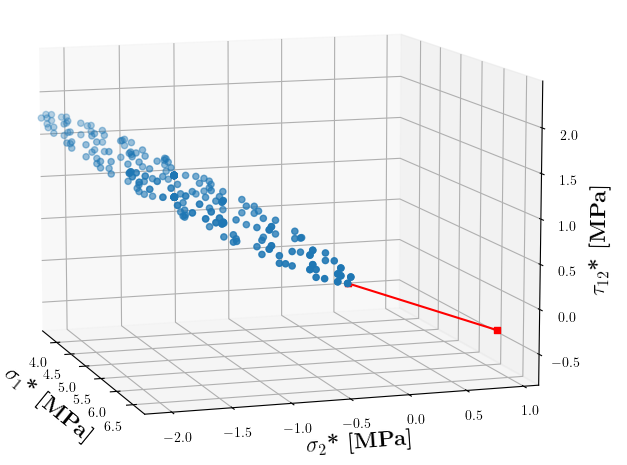
\includegraphics[width=0.5\textwidth]{ellipsoid_result.png}}
	\caption{And it works! The blue point cloud is the ideal ellipsoid. Its parameters were computed using the actual elastic parameters in table 1. The red square is the arbitrary outside point ($y$) and the red triangle is the point found by the algorithm ($x$). The red line links the outside point and its projection onto the ellispoid. }
	\label{fig2}
\end{figure}
\bibliography{biblio}
\end{document}